\def\imagetop#1{\vtop{\null\hbox{#1}}}

\documentclass[conference]{IEEEtran}
\usepackage{amsmath,graphicx,enumerate}
\usepackage{multirow}

% correct bad hyphenation here
\hyphenation{op-tical net-works semi-conduc-tor IEEEtran}

\IEEEoverridecommandlockouts    % to create the author's affliation portion

                % using \thanks

\textwidth 178mm    % <------ These are the adjustments we made 10/18/2005
\textheight 239mm   % You may or may not need to adjust these numbes again
\oddsidemargin -7mm
\evensidemargin -7mm
\topmargin -6mm
\columnsep 5mm

\begin{document}
\title{\ \\ \LARGE\bf Novelty Detection in Developmental Networks}
\author{Jordan Fish and Lisa Ossian}
\maketitle

\begin{abstract}
Neural networks traditionally have difficulty distinguishing between expected and unexpected novelty [1] due to the fuzzy, ill-defined boundaries between classes in traditional neural networks. We have extended the developmental network proposed by Weng [2] to have each neuron estimate the expected uncertainty inherent in their input patterns. Knowing the expected uncertainty allows the development network to predict whether a given query pattern is within expected uncertainty for a neuron or a novel pattern.
\end{abstract}

\begin{IEEEkeywords}
developmental network, rejection, novelty
\end{IEEEkeywords}

\section{Introduction}
Neurotransmitters are chemicals that allow the transmission of signals across synapses from one neuron to another. In the brain, several classes of neurotransmitters are used to connect one neuron to multiple neurons; this is called neural modulation. Neural modulation is needed in the brain to indicate certain properties about
sensory and motor signals \cite{cit:2}. Brains without neural modulation simply
respond to these signals and are not aware of the underlying properties that exist between them. This can be observed in children with ADHD who have trouble paying attention to detail. Neurons that are capable of neural modulation, such as acetylcholine and norepinephrine, are called neural modulators.

Yu \& Dayan \cite{cit:1} proposed that acetylcholine indicates expected uncertainty, while norepinephrine indicates unexpected uncertainty. Expected uncertainty is the known unreliability that occurs in a familiar environment, one in which a network has had a lot of experience. Unexpected uncertainty, or novelty, is the strongly unexpected observations that occur in an unfamiliar environment. Novelty is important to detect in neural networks, since it is impossible to train a neural network on all possible input.

Markou \& Singh \cite{cit:3} identified the main criterion for evaluating neural-network-based approaches to novelty detection as the maximization of true positives, or correctly-identified, novel input patterns, along with the minimization of false positives, or incorrectly-identified, novel input patterns. There are a number of neural-network-based approaches to novelty detection that perform well by this criterion. For instance, Ryan et al. \cite{cit:4} threshold the output of a neural network and detect novelty from low confidence, and Singh \& Markou \cite{cit:5} close known class boundaries, identify novel samples with their rejection filter, cluster these samples, and compare the clusters with known class distributions to determine whether they are outliers. However, both of these methods were implemented on multi-layer feed forward neural networks, or multi-layer perceptron. There was not a approach to novelty detection on a developmental network.

In the work presented in this paper, we extend the developmental network proposed by Weng \cite{cit:2} to be a neuromorphic system using acetylcholine and norepinephrine to detect novelty in input patterns. The developmental network presented performs facial recognition.  

\section{Theory}
Weng \cite{cit:2} introduced the theory for the neuromorphic, or emergent neuromodulation, system of acetylcholine (Ach) and norepinephrine (NE). Each neuron conducts synaptic maintenance, maintaining its synapses based on expected uncertainty, modeled by Ach, and unexpected uncertainty, modeled by NE. The goal of synaptic maintenance is to maximize the removal of irrelevant post-synaptic neurons, while minimizing the removal of relevant post-synaptic neurons, which in effect isolates the important information from the input.

The input to each neuron is in the form $\mathbf{p}=(p_1,p_2,\dots,p_d)$ and its synaptic weight vector is represented by $\mathbf{v}=(v_1,v_2,\dots,v_d)$.

The synapse of a firing top-k neuron $y$ contains information from the mean of the pre-synaptic activities, or input patterns, $x_i$. This can be written as:
\begin{align}v_i=E[yp_i\; | \;\text{the neuron fires}] \end{align}
which is calculated using the amnesic average \cite{cit:2}. Expected uncertainty is measured for each synapse $i$ by calculating the standard deviation of the match between $v_i$ and $p_i$:
\begin{align}\sigma_i=E[|v_i-p_i|\;|\;\text{the neuron fires}]\end{align}

Ach needs to be calculated incrementally and stably. The measure of unexpected uncertainty in equation (2) must be initialized with constant values and must wait until all synaptic weights have sufficient estimates of $w_i$. Letting $n$ represent the firing age of the neuron, for each synapse $n \le n_0$, the synapse is initialized to the standard deviation of the uniform distribution in $[-\delta,\delta]$. This standard deviation needs to be plastic continuously, so a constant asymptotic learning rate is used. Letting $\sigma_i(n)$ represent $\sigma_i$ at firing age $n$, synapse deviation is computed incrementally as follows:
\begin{align}\sigma_i(n)=\left\{
\begin{array}{l l}
\delta/\sqrt{12} &\text{if $n \le n_0$}\\
w_1(n)\sigma_i(n)+w_2(n)|v_i-p_i| & \text{otherwise}
\end{array}\right.\end{align}
where $w_1(n)$ is the retention rate and $w_2(n)$ is the learning rate, given by:
\begin{align}w_2(n)=\frac{1+\mu(n)}{n},w_1(n)=1-w_2(n). \nonumber \end{align}
To ensure sufficient estimates of synaptic weights through the first $n_0$ updates, set $n_0=20$. 

A neuron conducts synaptic maintenance based on the following equation for the expected goodness of match:
\begin{align}\bar{\sigma}(n)=\frac{1}{d}\sum_{i=1}^d\sigma_i(n)\end{align}
$\bar{\sigma}(n)$ represents the expected synaptic deviation among all of a neuron's synapses.

If $\sigma_i(n)$ is large, synapse $i$ should be retracted; however, setting a hard threshold may cause synapses to be retracted and extracted more than once. So a smooth synaptogenic factor $f(r)$ is defined, which is dependent on the relative synaptic deviation $r(n)$:
\begin{align}r_i(n)=\frac{\sigma_i(n)}{\bar{\sigma}(n)}\end{align}
\begin{align}
f(r)=\left\{
\begin{array}{l l}
1 & \text{if $r < \beta_s$} \\
(\beta_b-r)/(\beta_b-\beta_s) & \text{if $\beta_s \le r \le \beta_b$} \\
0 & \text{otherwise}
\end{array}\right.\end{align}
where $\beta_s=1.0$ and $\beta_b=1.5$. If all synapses match perfectly, then for all $i$, $r_i(n)=1$ and $f(r_i(n))=1$; in this case, no synapses should be cut. In the case where all synapses do not match perfectly, synapses with $r_i(n) < \beta_s$ are fully operational, synapses with $\beta_s < r_i(n) < \beta_b$ are partially cut, and synapses with $\beta_b < r_i(n)$ are completely cut. Weng \cite{cit:2} hypothesized that synapses with $\beta_b < r_i(n)$ indicate novelty. For input patterns that produce $\beta_b < r_i(n)$ in a synapse, the developmental network needs to reject.

\section{Algorithm}
The development network was implemented using Python 2.7 using NumPy 1.61 for vector math functions.  The deviation from the expected input was computed for each neuron at each synapse in each layer during supervised training.  The expected deviation was only updated when a neuron fired and the network was not allowed to reject input during the training phase.

When testing, for each input pattern the top k firing neurons estimated the deviation from the expected value for each synapse.  Each dimension in the input whose $r$-value that was below a threshold $R$ was counted.  If the ratio of dimensions that had unexpected novelty to the total number of dimensions was larger than a threshold $\theta$ the neuron’s firing was suppressed.  This suppression was done in the Y layer only.

For the first training epoch the input images were ordered such that the network was presented one view of each person before seeing a new view of the same person, this was done to speed up training convergence.  For subsequent training epochs the images were presented to the network in a random order.

\section{Experimental Results}
For evaluating the network the admissible and not admissible set were created based on the idea that during any given day a person encounters many more faces of people they do not know (faces that the network should reject) than faces they do know.  Additionally the people encountered can be very well known (many training views) or only a casual acquaintance (few training views).  Admissible and not admissible images were selected from a set of a total of 1825 views of 188 people.  For the admissible set 14 people totalling 187 views were selected and used to train the network. The number of views for each individual ranging from 6 to 53. \ref{fig:training} shows the first view of the 14 people used to train the network and the number of views for each individual; person one is in the top left corner through person 14 in the lower right. The testing set consisted of 1638 views over all 188 people in the dataset.  Of these there were 295 views of the 14 people in the admissible set on and 1343 views of 174 people in the not admissible set.  

\begin{figure}
\center
\fontsize{8}{12}\selectfont
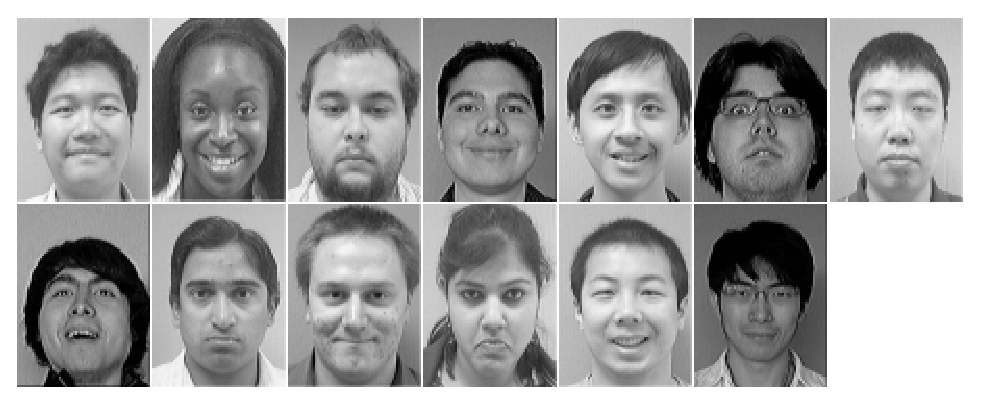
\includegraphics[width=3in]{training_faces.eps}
\begin{tabular}{c} \\[3ex] \end{tabular}
\begin{tabular}{|c|c|}
  \hline
  Person & Number of views\\
  \hline
  1 & 6\\
  2 & 7\\
  3 & 6\\
  4 & 22\\
  5 & 9\\
  6 & 16\\
  7 & 7\\
  8 & 22\\
  9 & 7\\
  10 & 7\\
  11 & 8\\
  12 & 7\\
  13 & 10\\
  14 & 53\\
  \hline
\end{tabular}
\caption{First view of the 14 people in the admissible set and the number of views for each person.  Person one is in the top left corner through person 14 in the lower right.}
\label{fig:training}
\end{figure}

The development network was built using 25 neurons in the Y layer and trained over 50 epochs of the training images.  For each epoch the optimal value for $R$ and $\theta$ were searched for using the grid search technique.  The search was performed over a subset of the input parameter space $R=[0.05-0.90]$ and $\theta=[0.05-0.90]$.  The sensitivity and specificity for each pair of values $R$ and $\theta$ were computed and plotted in a Receiver Operating Characteristics Curve, five representative epochs of which can be seen in \ref{fig:roc}. The network rapidly stabilized and achieved the best accuracy, $95.8\%$ after the third training epoch.  After the sixth training epoch the network achieved it's maximum sensitivity and specificity of $96.6\%$ and $92.5\%$ respectively with $R=.4$ and $\theta=.35$ and had an accuracy of $91.9\%$.  Beyond this point the sensitivity and specificity drop as the network began to over fit the training data.  

\begin{figure}
\center
\fontsize{8}{12}\selectfont
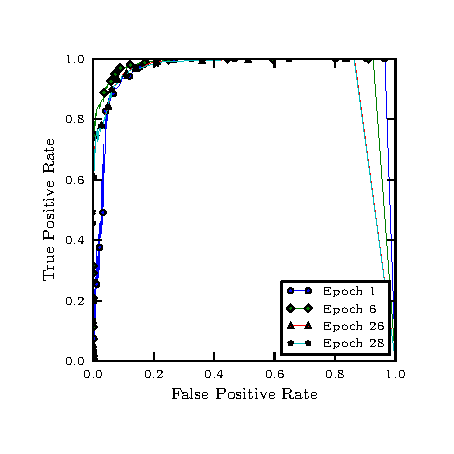
\includegraphics[width=2.75in]{5_yneuron/roc.eps}
\caption{Receiver operating characteristic (ROC) curve for training epochs 1, 6, 9 and 26.  This figure shows how the sensitivity and specificity increase with the number of training epochs (curves shifting closer to the upper right hand corner) then fall off after the network begins over fitting.}
\label{fig:roc}
\end{figure}

The sixth training epoch, where the highest sensitivity and specificity were achieved, was analyzed further.  First the pre-synaptic weights for the $Y$ and $Z$ layer were visualized.  \ref{fig:y_weights} shows the pre-synaptic weights for the Y layer; these images are essentially averages of the input images that each neuron responds to.  Then the expected variation for each Y neuron, $\sigma$ was plotted in \ref{fig:y_sigmas}.  Each pixel represented the amount of variation the specific $Y$ neuron expects from the $X$ layer neuron.  Darker pixels represent lower expected variation while lighter pixels represent inputs with higher expected variation.  Of note is the first Y neuron, which is trained to respond to the background image that is presented before each classification task.  The image is a picture of the background each person had their picture taken against and the same image was presented each time which is why the expected variation is 0, an all black image.  For the Z layer the pre-synaptic weights for each of plotted in \ref{fig:z_weights} 5 per line. The lighter a square is the higher the weight for that Y neuron.  The firing ages for each of the Y and Z neurons were graphed in \${fig:ages} which showed that three neurons (neurons 2, 11, and 22) were under-utilized, responding to only a single view from the admissible set.  This is also shown in \ref{fig:y_sigmas} as the black squares, representing no expected variation in the input for those neurons.

\begin{figure}
\center
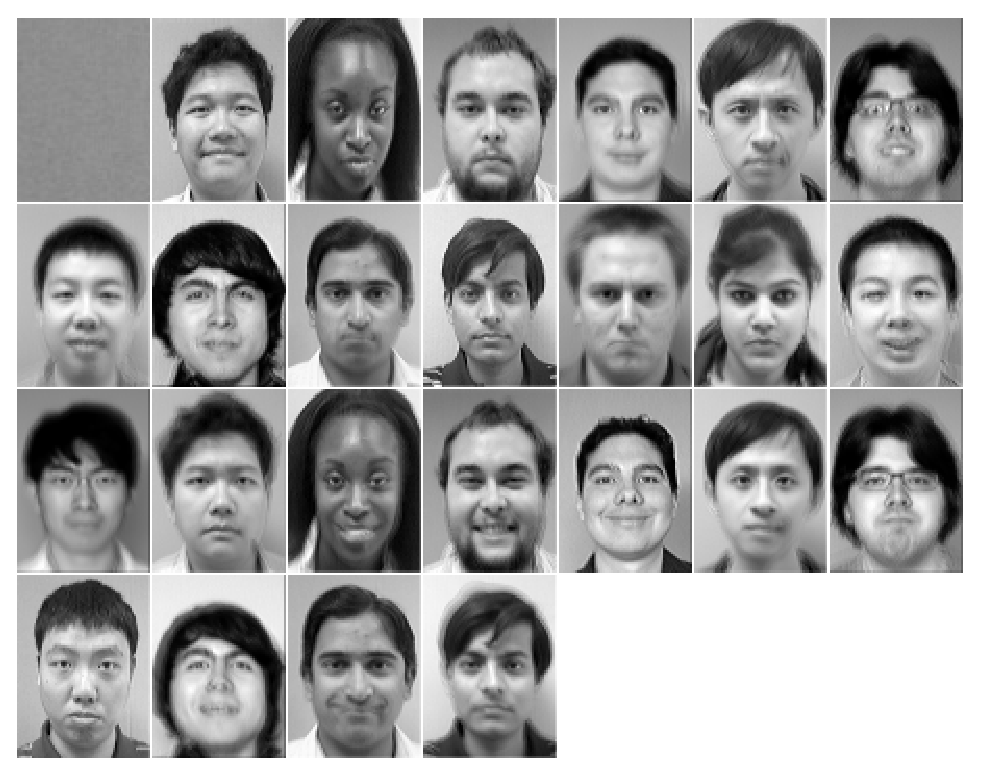
\includegraphics[width=3in]{5_yneuron/epoch_5_0_xy.eps}
\caption{Visualization of pre-synaptic weights for the 25 Y layer neurons after the sixth training epoch, the first image corresponds to the Y neuron that responds to the background image presented to the network before every classification face.}
\label{fig:y_weights}
\end{figure}

\begin{figure}
\center
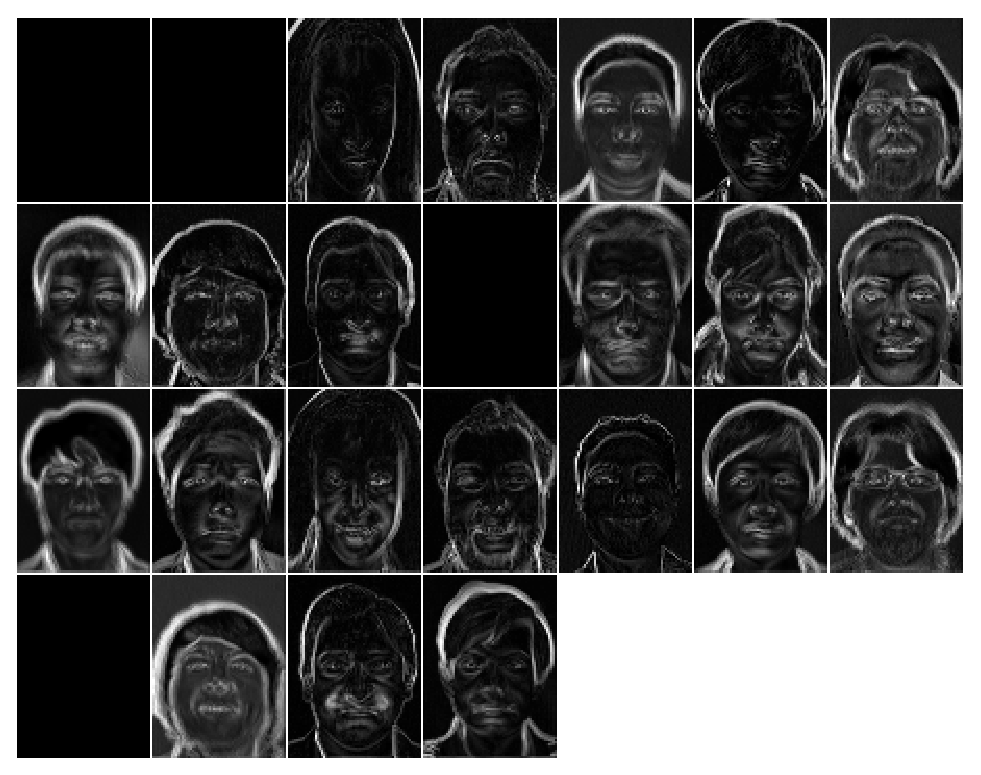
\includegraphics[width=3in]{5_yneuron/epoch_5_0_sigmas.eps}
\caption{Visualization of the expected variance for each of the 25 neurons in the Y layer after the sixth training epoch.  The darker areas show inputs from the X layer where little variation is expected while the white areas show inputs that are expected to have larger variation.  Four neurons: 1, 2, 10, 22 (all black images) had no expected variation.}
\label{fig:y_sigmas}
\end{figure}

\begin{figure}
\center

\includegraphics[width=3in]{5_yneuron/epoch_5_0_yz.eps}
\caption{Visualization of pre-synaptic weights for Z layer neurons after the sixth training epoch.  Each square represents a Z neuron.  The 25 pixels in each of the 25x25 squares represents the response weight for the corresponding Y neuron, the lighter the pixel the higher the weight.}
\label{fig:z_weights}
\end{figure}

\begin{figure}
\center
\fontsize{8}{12}\selectfont
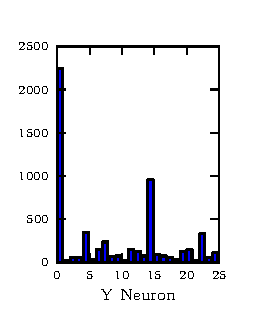
\includegraphics{5_yneuron/epoch_5_y_ages.eps}
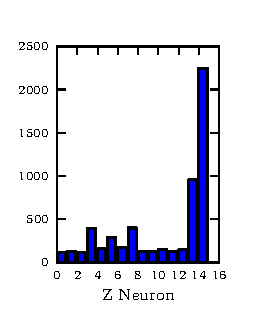
\includegraphics{5_yneuron/epoch_5_z_ages.eps}
\caption{Plot of Y (left) and Z (right) neuron firing ages after the sixth training epoch.  The first (left most) Y neuron and last (right most) Z neuron are the neurons trained to respond to the background image that is presented before every image, which is why the firing rate for those neurons are higher than the rest.}
\label{fig:ages}
\end{figure}

Finally for the sixth epoch the 126 errors the network made when using the parameters $R=.4$ and $\theta=.35$ were broken down by error type: false acceptance, false rejection, and incorrect classification. Of the 126 errors a large number were duplicates of the same error, incorrectly classifying multiple views of the same person in to the same category.  Consolidating the errors down to one person input person-incorrect classification pair there were 3 false acceptances, 7 false rejections, and 2 incorrect classifications as seen in \ref{fig:6_epoch_errors}.  The falsely accepted faces on visual inspect appear very similar to people in the training set.  The false rejections appear to be a combination of mismatched white-balancing and errors made due to different facial expressions.  The mistakes appear to be due to facial expressions and orientations different from the learned faces.  The incorrect classifications and false rejections due to facial expressions can be improved by increasing the number of neurons in the Y layer.

\begin{figure}
\center
\begin{tabular}{cc}
\fontsize{8}{12}\selectfont
a \imagetop{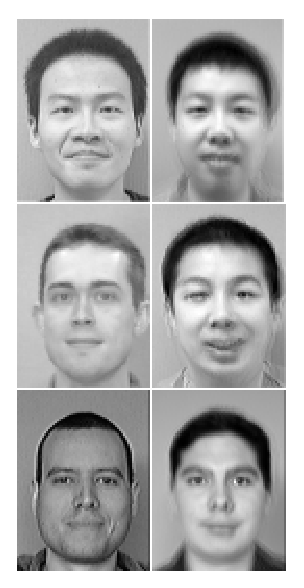
\includegraphics[width=1.4in]{5_yneuron/false_accept_combined.eps}} &
\multirow{2}{*}{b \imagetop{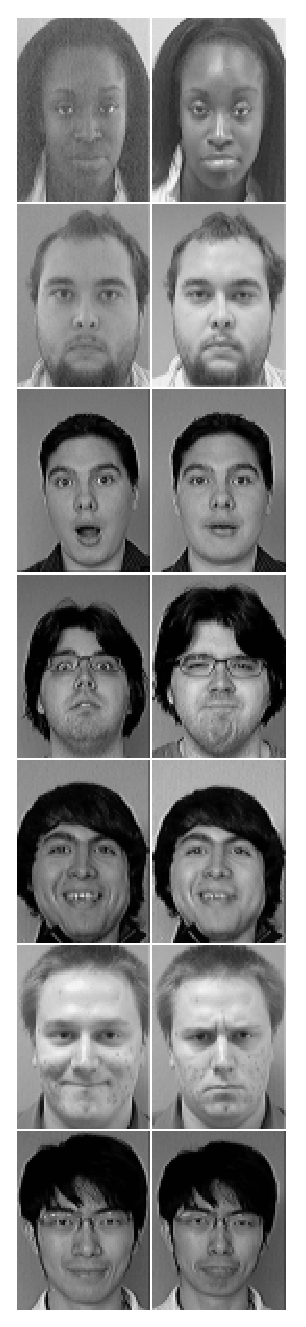
\includegraphics[width=1.4in]{5_yneuron/false_reject_combined.eps}}} \\
c \imagetop{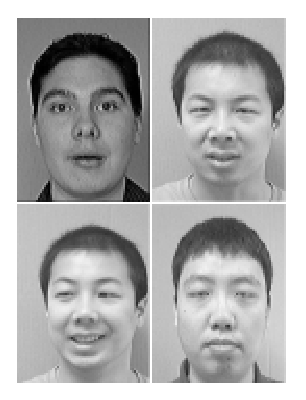
\includegraphics[width=1.4in]{5_yneuron/mistakes_combined.eps}} & \\[60ex]
\end{tabular}
\caption{a. The incorrectly accepted image (on the left) compared to the y neuron pre-synaptic weights for the Y neuron with the highest response to the input image. b. Input image (left) compared to the first input face for the falsely rejected images. c. The input image (left) and view of the person (right) the network labeled the two misclassified people as.}
\label{fig:6_epoch_errors}
\end{figure}

\section{Conclusion}
In conclusion, existing neural networks have difficulties in identifying novel patterns.  The development network proposed by Weng et al. (citation) provides a strong foundation for new neural networks with enhanced capabilities.  By learning not only the patterns that come from each class but the expected distribution of the patterns this neural network is able to detect novel input patterns.
\newpage
\begin{thebibliography}{1}
\bibitem{cit:1} A. J. Yu and P. Dayan.{\it  Uncertainty, neuromodulation, and attention}. Neuron, 46:681-692, 2005.
\bibitem{cit:2} J. Weng. {\it Natural and Artificial Intelligence}. BMI Press, East Lansing, 2012.
\bibitem{cit:3} M. Markou and S. Singh. {\it Novelty detection: a review - part 2: neural network based approaches.} Signal Processing, 83(12):2499-2521, 2003.
\bibitem{cit:4} J. Ryan, M. Lin, and R. {\it Miikkulainen. Intrusion detection with neural networks.} Advances in Neural Information Processing Systems, 10:943-949, 1998.
\bibitem{cit:5} S. Singh, M. Markou, {\it An approach to novelty detection applied to the classification of image regions.} IEEE Transactions on Knowledge and Data Engineering, 16(4):396-407, 2004.
\end{thebibliography}

\end{document}
